\documentclass[]{article}
\usepackage{lmodern}
\usepackage{amssymb,amsmath}
\usepackage{ifxetex,ifluatex}
\usepackage{fixltx2e} % provides \textsubscript
\ifnum 0\ifxetex 1\fi\ifluatex 1\fi=0 % if pdftex
  \usepackage[T1]{fontenc}
  \usepackage[utf8]{inputenc}
\else % if luatex or xelatex
  \ifxetex
    \usepackage{mathspec}
  \else
    \usepackage{fontspec}
  \fi
  \defaultfontfeatures{Ligatures=TeX,Scale=MatchLowercase}
\fi
% use upquote if available, for straight quotes in verbatim environments
\IfFileExists{upquote.sty}{\usepackage{upquote}}{}
% use microtype if available
\IfFileExists{microtype.sty}{%
\usepackage[]{microtype}
\UseMicrotypeSet[protrusion]{basicmath} % disable protrusion for tt fonts
}{}
\PassOptionsToPackage{hyphens}{url} % url is loaded by hyperref
\usepackage[unicode=true]{hyperref}
\hypersetup{
            pdftitle={Survival and Weights of Pups of First Parity Mice},
            pdfauthor={Noura El Habbal},
            pdfborder={0 0 0},
            breaklinks=true}
\urlstyle{same}  % don't use monospace font for urls
\usepackage[margin=1in]{geometry}
\usepackage{longtable,booktabs}
% Fix footnotes in tables (requires footnote package)
\IfFileExists{footnote.sty}{\usepackage{footnote}\makesavenoteenv{long table}}{}
\usepackage{graphicx,grffile}
\makeatletter
\def\maxwidth{\ifdim\Gin@nat@width>\linewidth\linewidth\else\Gin@nat@width\fi}
\def\maxheight{\ifdim\Gin@nat@height>\textheight\textheight\else\Gin@nat@height\fi}
\makeatother
% Scale images if necessary, so that they will not overflow the page
% margins by default, and it is still possible to overwrite the defaults
% using explicit options in \includegraphics[width, height, ...]{}
\setkeys{Gin}{width=\maxwidth,height=\maxheight,keepaspectratio}
\IfFileExists{parskip.sty}{%
\usepackage{parskip}
}{% else
\setlength{\parindent}{0pt}
\setlength{\parskip}{6pt plus 2pt minus 1pt}
}
\setlength{\emergencystretch}{3em}  % prevent overfull lines
\providecommand{\tightlist}{%
  \setlength{\itemsep}{0pt}\setlength{\parskip}{0pt}}
\setcounter{secnumdepth}{5}
% Redefines (sub)paragraphs to behave more like sections
\ifx\paragraph\undefined\else
\let\oldparagraph\paragraph
\renewcommand{\paragraph}[1]{\oldparagraph{#1}\mbox{}}
\fi
\ifx\subparagraph\undefined\else
\let\oldsubparagraph\subparagraph
\renewcommand{\subparagraph}[1]{\oldsubparagraph{#1}\mbox{}}
\fi

% set default figure placement to htbp
\makeatletter
\def\fps@figure{htbp}
\makeatother


\title{Survival and Weights of Pups of First Parity Mice}
\author{Noura El Habbal}
\date{2020}

\begin{document}
\maketitle

{
\setcounter{tocdepth}{2}
\tableofcontents
}
\section{Raw Data}\label{raw-data}

\begin{longtable}[]{@{}rllrlrlrrrrr@{}}
\caption{Average Births and Survival Rates per Cage}\tabularnewline
\toprule
MaternalID & MaternalGenotype & BirthDate & Dead & na.rm & Total & is.na
& Litter & Alive & alive.percent & survival.rate &
Average.Births.Per.Litter\tabularnewline
\midrule
\endfirsthead
\toprule
MaternalID & MaternalGenotype & BirthDate & Dead & na.rm & Total & is.na
& Litter & Alive & alive.percent & survival.rate &
Average.Births.Per.Litter\tabularnewline
\midrule
\endhead
7981 & KO & 6/8/19 & 0 & TRUE & 5 & NA & 1 & 5 & 100.0 & 1.000 &
5\tabularnewline
7982 & WT & 6/20/19 & 0 & TRUE & 7 & NA & 1 & 7 & 100.0 & 1.000 &
7\tabularnewline
7983 & KO & 6/7/19 & 0 & TRUE & 3 & NA & 1 & 3 & 100.0 & 1.000 &
3\tabularnewline
7984 & KO & 6/9/19 & 0 & TRUE & 6 & NA & 1 & 6 & 100.0 & 1.000 &
6\tabularnewline
8161 & KO & 6/6/19 & 0 & TRUE & 8 & NA & 1 & 8 & 100.0 & 1.000 &
8\tabularnewline
8162 & WT & 6/5/19 & 0 & TRUE & 7 & NA & 1 & 7 & 100.0 & 1.000 &
7\tabularnewline
8444 & WT & 7/5/19 & 1 & TRUE & 9 & NA & 1 & 8 & 88.9 & 0.889 &
9\tabularnewline
8445 & WT & 7/6/19 & 0 & TRUE & 8 & NA & 1 & 8 & 100.0 & 1.000 &
8\tabularnewline
8446 & WT & 7/8/19 & 0 & TRUE & 9 & NA & 1 & 9 & 100.0 & 1.000 &
9\tabularnewline
8465 & KO & 7/8/19 & 0 & TRUE & 7 & NA & 1 & 7 & 100.0 & 1.000 &
7\tabularnewline
8466 & KO & 7/3/19 & 1 & TRUE & 10 & NA & 1 & 9 & 90.0 & 0.900 &
10\tabularnewline
8467 & WT & 7/6/19 & 0 & TRUE & 7 & NA & 1 & 7 & 100.0 & 1.000 &
7\tabularnewline
\bottomrule
\end{longtable}

\begin{longtable}[]{@{}lrrr@{}}
\caption{Average Survival per Genotype}\tabularnewline
\toprule
MaternalGenotype & Average.Survival & SE.Average.Survival &
Number\tabularnewline
\midrule
\endfirsthead
\toprule
MaternalGenotype & Average.Survival & SE.Average.Survival &
Number\tabularnewline
\midrule
\endhead
WT & 98.1 & 1.85 & 6\tabularnewline
KO & 98.3 & 1.67 & 6\tabularnewline
\bottomrule
\end{longtable}

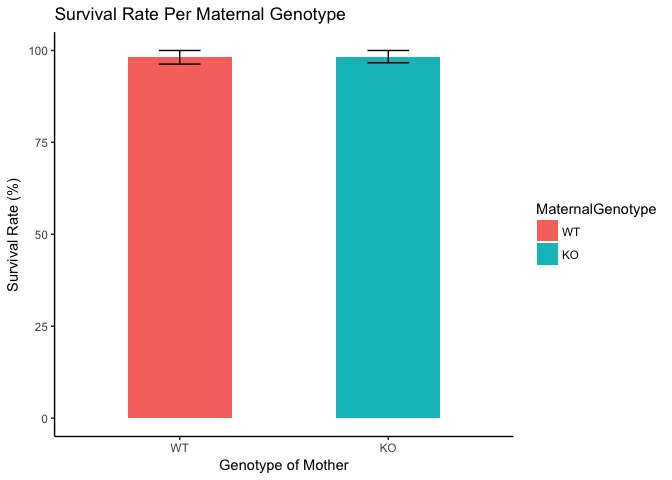
\includegraphics{figures/atsc-survivalpergenotype-bargraph-1.png}

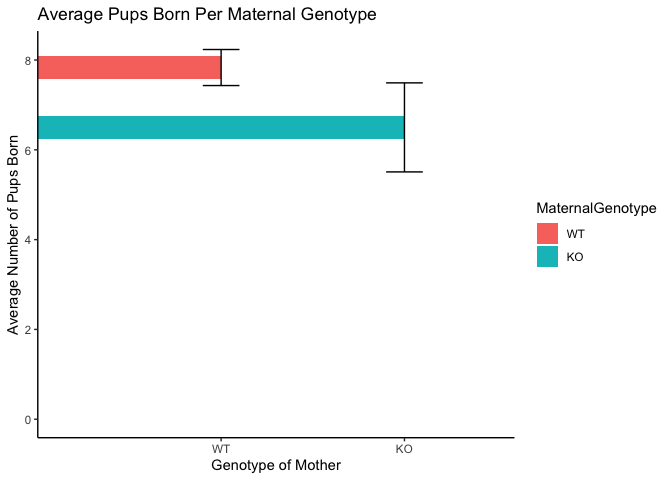
\includegraphics{figures/numberofpupspergenotype-1.png}
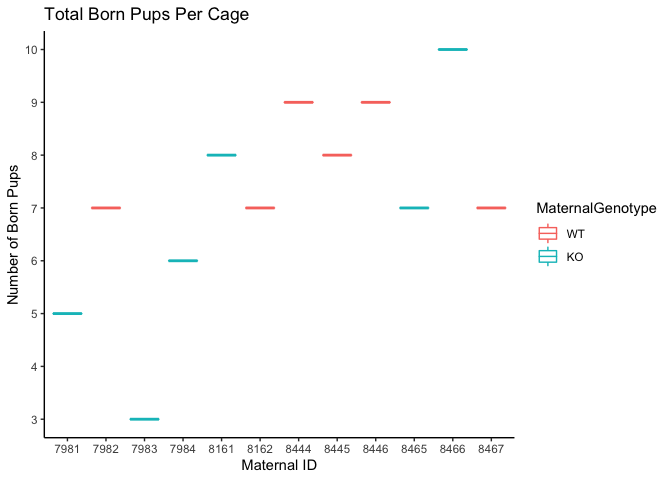
\includegraphics{figures/numberofpupspergenotype-2.png}

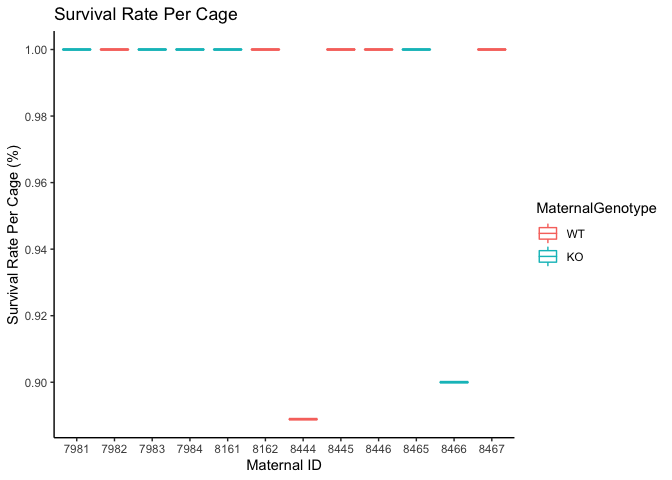
\includegraphics{figures/atsc-fertilitypercage-bargraph-1.png}
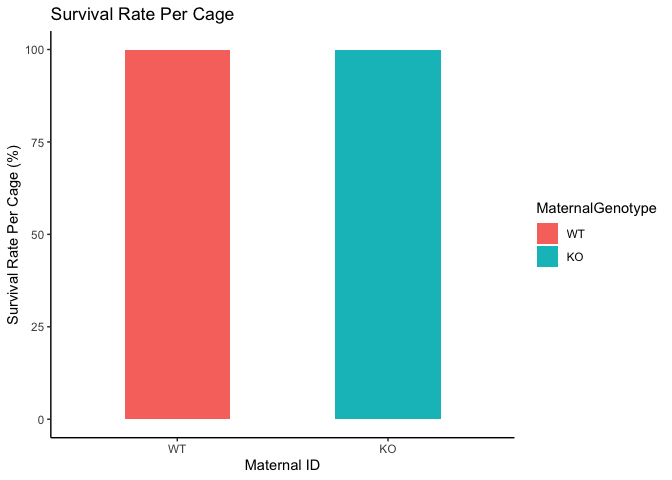
\includegraphics{figures/atsc-fertilitypercage-bargraph-2.png}
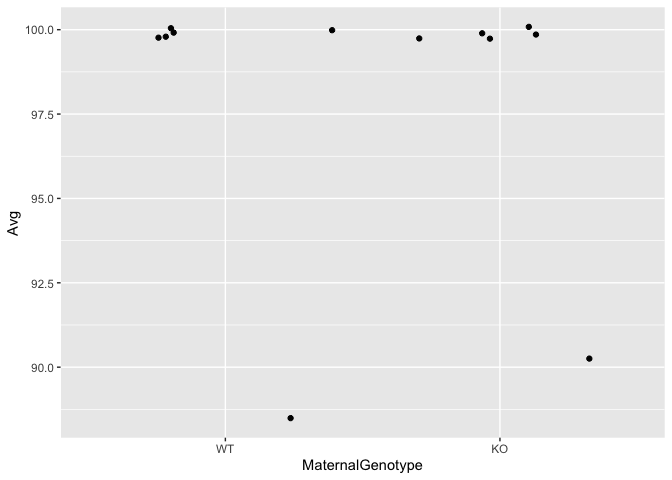
\includegraphics{figures/atsc-fertilitypercage-bargraph-3.png}

\begin{longtable}[]{@{}rlrrrrl@{}}
\toprule
MaternalID & MaternalGenotype & Average.Weight & SE.Average.Weight &
Average.size & Total & is.na\tabularnewline
\midrule
\endhead
7981 & KO & 1.44 & 0.016 & 5 & 5 & NA\tabularnewline
7982 & WT & 1.33 & 0.026 & 7 & 7 & NA\tabularnewline
7983 & KO & 1.47 & 0.058 & 3 & 3 & NA\tabularnewline
7984 & KO & 1.35 & 0.021 & 6 & 6 & NA\tabularnewline
8161 & KO & 1.23 & 0.025 & 8 & 8 & NA\tabularnewline
8162 & WT & 1.29 & 0.045 & 7 & 7 & NA\tabularnewline
8444 & WT & 1.32 & 0.017 & 8 & 8 & NA\tabularnewline
8445 & WT & 1.26 & 0.021 & 8 & 8 & NA\tabularnewline
8446 & WT & 1.24 & 0.024 & 9 & 9 & NA\tabularnewline
8465 & KO & 1.38 & 0.024 & 7 & 7 & NA\tabularnewline
8466 & KO & 1.31 & 0.030 & 9 & 9 & NA\tabularnewline
8467 & WT & 1.28 & 0.033 & 7 & 7 & NA\tabularnewline
\bottomrule
\end{longtable}

\begin{longtable}[]{@{}lrrrrl@{}}
\toprule
MaternalGenotype & Average.Weight & SE.Average.Weight & Average.size &
Total & is.na\tabularnewline
\midrule
\endhead
WT & 1.29 & 0.004 & 1 & 1 & NA\tabularnewline
KO & 1.36 & 0.006 & 1 & 1 & NA\tabularnewline
\bottomrule
\end{longtable}

\begin{longtable}[]{@{}lrrrrr@{}}
\toprule
term & df & sumsq & meansq & statistic & p.value\tabularnewline
\midrule
\endhead
MaternalGenotype & 1 & 0.018 & 0.018 & 3.97 & 0.074\tabularnewline
Residuals & 10 & 0.045 & 0.005 & NA & NA\tabularnewline
\bottomrule
\end{longtable}

\begin{longtable}[]{@{}rllrrrrl@{}}
\toprule
MaternalID & MaternalGenotype & Sex & Average.Weight & SE.Average.Weight
& Average.size & Total & is.na\tabularnewline
\midrule
\endhead
7981 & KO & Female & 4.20 & 0.000 & 2 & 2 & NA\tabularnewline
7981 & KO & Male & 4.25 & 0.150 & 2 & 2 & NA\tabularnewline
7983 & KO & Female & 4.70 & 0.100 & 2 & 2 & NA\tabularnewline
7983 & KO & Male & 4.30 & NA & 1 & 1 & NA\tabularnewline
7984 & KO & Female & 4.40 & NA & 1 & 1 & NA\tabularnewline
7984 & KO & Male & 4.10 & 0.058 & 3 & 3 & NA\tabularnewline
8161 & KO & Female & 3.95 & 0.050 & 2 & 2 & NA\tabularnewline
8161 & KO & Male & 4.15 & 0.050 & 2 & 2 & NA\tabularnewline
8162 & WT & Female & 3.65 & 0.050 & 2 & 2 & NA\tabularnewline
8162 & WT & Male & 3.90 & 0.100 & 2 & 2 & NA\tabularnewline
8444 & WT & Female & 4.10 & 0.000 & 2 & 2 & NA\tabularnewline
8444 & WT & Male & 4.10 & 0.000 & 2 & 2 & NA\tabularnewline
8445 & WT & Female & 4.00 & 0.100 & 2 & 2 & NA\tabularnewline
8445 & WT & Male & 4.05 & 0.050 & 2 & 2 & NA\tabularnewline
8446 & WT & Female & 4.35 & 0.150 & 2 & 2 & NA\tabularnewline
8446 & WT & Male & 4.25 & 0.150 & 2 & 2 & NA\tabularnewline
8465 & KO & Female & 4.35 & 0.250 & 2 & 2 & NA\tabularnewline
8465 & KO & Male & 4.15 & 0.150 & 2 & 2 & NA\tabularnewline
8466 & KO & Female & 4.50 & 0.000 & 2 & 2 & NA\tabularnewline
8466 & KO & Male & 4.65 & 0.050 & 2 & 2 & NA\tabularnewline
8467 & WT & Female & 3.77 & 0.131 & 4 & 4 & NA\tabularnewline
\bottomrule
\end{longtable}

\begin{longtable}[]{@{}llrrrrl@{}}
\toprule
MaternalGenotype & Sex & Average.Weight & SE.Average.Weight &
Average.size & Total & is.na\tabularnewline
\midrule
\endhead
WT & Female & 3.98 & 0.027 & 1 & 1 & NA\tabularnewline
WT & Male & 4.08 & 0.032 & 1 & 1 & NA\tabularnewline
KO & Female & 4.35 & 0.042 & 1 & 1 & NA\tabularnewline
KO & Male & 4.27 & 0.022 & 1 & 1 & NA\tabularnewline
\bottomrule
\end{longtable}

\begin{longtable}[]{@{}lrrrrr@{}}
\toprule
term & df & sumsq & meansq & statistic & p.value\tabularnewline
\midrule
\endhead
MaternalGenotype & 1 & 0.429 & 0.429 & 8.208 & 0.010\tabularnewline
Sex & 1 & 0.000 & 0.000 & 0.003 & 0.958\tabularnewline
Residuals & 18 & 0.941 & 0.052 & NA & NA\tabularnewline
\bottomrule
\end{longtable}

\begin{longtable}[]{@{}lrrrrr@{}}
\toprule
term & df & sumsq & meansq & statistic & p.value\tabularnewline
\midrule
\endhead
MaternalGenotype & 1 & 0.429 & 0.429 & 8.122 & 0.011\tabularnewline
Sex & 1 & 0.000 & 0.000 & 0.003 & 0.958\tabularnewline
MaternalGenotype:Sex & 1 & 0.043 & 0.043 & 0.812 & 0.380\tabularnewline
Residuals & 17 & 0.898 & 0.053 & NA & NA\tabularnewline
\bottomrule
\end{longtable}

\begin{longtable}[]{@{}rllrrrrl@{}}
\toprule
MaternalID & MaternalGenotype & Sex & Average.Weight & SE.Average.Weight
& Average.size & Total & is.na\tabularnewline
\midrule
\endhead
7981 & KO & Female & 7.95 & 0.050 & 2 & 2 & NA\tabularnewline
7981 & KO & Male & 8.05 & 0.050 & 2 & 2 & NA\tabularnewline
7983 & KO & Female & 9.05 & 0.150 & 2 & 2 & NA\tabularnewline
7983 & KO & Male & 7.20 & NA & 1 & 1 & NA\tabularnewline
7984 & KO & Female & 6.20 & NA & 1 & 1 & NA\tabularnewline
7984 & KO & Male & 7.77 & 0.088 & 3 & 3 & NA\tabularnewline
8161 & KO & Female & 7.25 & 0.150 & 2 & 2 & NA\tabularnewline
8161 & KO & Male & 7.70 & 0.100 & 2 & 2 & NA\tabularnewline
8162 & WT & Female & 7.15 & 0.150 & 2 & 2 & NA\tabularnewline
8162 & WT & Male & 7.20 & 0.100 & 2 & 2 & NA\tabularnewline
8444 & WT & Female & 8.05 & 0.150 & 2 & 2 & NA\tabularnewline
8444 & WT & Male & 7.95 & 0.250 & 2 & 2 & NA\tabularnewline
8445 & WT & Female & 7.95 & 0.050 & 2 & 2 & NA\tabularnewline
8445 & WT & Male & 8.00 & 0.500 & 2 & 2 & NA\tabularnewline
8446 & WT & Female & 8.15 & 0.250 & 2 & 2 & NA\tabularnewline
8446 & WT & Male & 8.05 & 0.450 & 2 & 2 & NA\tabularnewline
8465 & KO & Female & 7.70 & 0.400 & 2 & 2 & NA\tabularnewline
8465 & KO & Male & 7.80 & 0.000 & 2 & 2 & NA\tabularnewline
8466 & KO & Female & 8.55 & 0.050 & 2 & 2 & NA\tabularnewline
8466 & KO & Male & 8.55 & 0.150 & 2 & 2 & NA\tabularnewline
8467 & WT & Female & 7.25 & 0.210 & 4 & 4 & NA\tabularnewline
\bottomrule
\end{longtable}

\begin{longtable}[]{@{}llrrrrl@{}}
\toprule
MaternalGenotype & Sex & Average.Weight & SE.Average.Weight &
Average.size & Total & is.na\tabularnewline
\midrule
\endhead
WT & Female & 7.71 & 0.034 & 1 & 1 & NA\tabularnewline
WT & Male & 7.80 & 0.092 & 1 & 1 & NA\tabularnewline
KO & Female & 7.78 & 0.058 & 1 & 1 & NA\tabularnewline
KO & Male & 7.84 & 0.023 & 1 & 1 & NA\tabularnewline
\bottomrule
\end{longtable}

\begin{longtable}[]{@{}lrrrrr@{}}
\toprule
term & df & sumsq & meansq & statistic & p.value\tabularnewline
\midrule
\endhead
MaternalGenotype & 1 & 0.021 & 0.021 & 0.051 & 0.824\tabularnewline
Sex & 1 & 0.028 & 0.028 & 0.069 & 0.796\tabularnewline
Residuals & 18 & 7.381 & 0.410 & NA & NA\tabularnewline
\bottomrule
\end{longtable}

\begin{longtable}[]{@{}lrrrrr@{}}
\toprule
term & df & sumsq & meansq & statistic & p.value\tabularnewline
\midrule
\endhead
MaternalGenotype & 1 & 0.021 & 0.021 & 0.048 & 0.829\tabularnewline
Sex & 1 & 0.028 & 0.028 & 0.065 & 0.802\tabularnewline
MaternalGenotype:Sex & 1 & 0.001 & 0.001 & 0.002 & 0.961\tabularnewline
Residuals & 17 & 7.380 & 0.434 & NA & NA\tabularnewline
\bottomrule
\end{longtable}

\begin{longtable}[]{@{}rllrrrrl@{}}
\toprule
MaternalID & MaternalGenotype & Sex & Average.Weight & SE.Average.Weight
& Average.size & Total & is.na\tabularnewline
\midrule
\endhead
7981 & KO & Female & 8.60 & 0.100 & 2 & 2 & NA\tabularnewline
7981 & KO & Male & 8.85 & 0.050 & 2 & 2 & NA\tabularnewline
7983 & KO & Female & 9.50 & 0.500 & 2 & 2 & NA\tabularnewline
7983 & KO & Male & 7.80 & NA & 1 & 1 & NA\tabularnewline
7984 & KO & Female & 6.90 & NA & 1 & 1 & NA\tabularnewline
7984 & KO & Male & 8.10 & 0.058 & 3 & 3 & NA\tabularnewline
8161 & KO & Female & 7.65 & 0.150 & 2 & 2 & NA\tabularnewline
8161 & KO & Male & 8.15 & 0.050 & 2 & 2 & NA\tabularnewline
8162 & WT & Female & 7.65 & 0.150 & 2 & 2 & NA\tabularnewline
8162 & WT & Male & 7.70 & 0.100 & 2 & 2 & NA\tabularnewline
8444 & WT & Female & 8.55 & 0.050 & 2 & 2 & NA\tabularnewline
8444 & WT & Male & 8.60 & 0.200 & 2 & 2 & NA\tabularnewline
8445 & WT & Female & 8.45 & 0.050 & 2 & 2 & NA\tabularnewline
8445 & WT & Male & 8.60 & 0.500 & 2 & 2 & NA\tabularnewline
8446 & WT & Female & 8.70 & 0.100 & 2 & 2 & NA\tabularnewline
8446 & WT & Male & 8.80 & 0.500 & 2 & 2 & NA\tabularnewline
8465 & KO & Female & 8.25 & 0.350 & 2 & 2 & NA\tabularnewline
8465 & KO & Male & 8.45 & 0.050 & 2 & 2 & NA\tabularnewline
8466 & KO & Female & 9.00 & 0.100 & 2 & 2 & NA\tabularnewline
8466 & KO & Male & 9.00 & 0.000 & 2 & 2 & NA\tabularnewline
8467 & WT & Female & 7.60 & 0.248 & 4 & 4 & NA\tabularnewline
\bottomrule
\end{longtable}

\begin{longtable}[]{@{}llrrrrl@{}}
\toprule
MaternalGenotype & Sex & Average.Weight & SE.Average.Weight &
Average.size & Total & is.na\tabularnewline
\midrule
\endhead
WT & Female & 8.19 & 0.037 & 1 & 1 & NA\tabularnewline
WT & Male & 8.43 & 0.103 & 1 & 1 & NA\tabularnewline
KO & Female & 8.32 & 0.073 & 1 & 1 & NA\tabularnewline
KO & Male & 8.39 & 0.010 & 1 & 1 & NA\tabularnewline
\bottomrule
\end{longtable}

\begin{longtable}[]{@{}lrrrrr@{}}
\toprule
term & df & sumsq & meansq & statistic & p.value\tabularnewline
\midrule
\endhead
MaternalGenotype & 1 & 0.018 & 0.018 & 0.045 & 0.834\tabularnewline
Sex & 1 & 0.107 & 0.107 & 0.262 & 0.615\tabularnewline
Residuals & 18 & 7.338 & 0.408 & NA & NA\tabularnewline
\bottomrule
\end{longtable}

\begin{longtable}[]{@{}lrrrrr@{}}
\toprule
term & df & sumsq & meansq & statistic & p.value\tabularnewline
\midrule
\endhead
MaternalGenotype & 1 & 0.018 & 0.018 & 0.043 & 0.839\tabularnewline
Sex & 1 & 0.107 & 0.107 & 0.249 & 0.624\tabularnewline
MaternalGenotype:Sex & 1 & 0.033 & 0.033 & 0.076 & 0.786\tabularnewline
Residuals & 17 & 7.305 & 0.430 & NA & NA\tabularnewline
\bottomrule
\end{longtable}

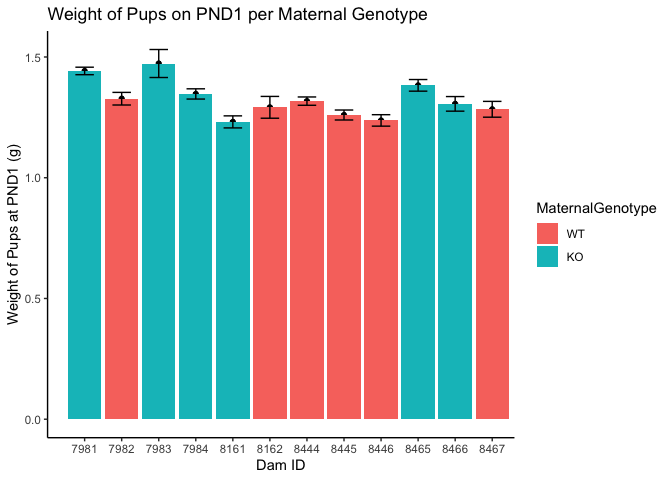
\includegraphics{figures/PUPweight_graphsPND1-1.png}
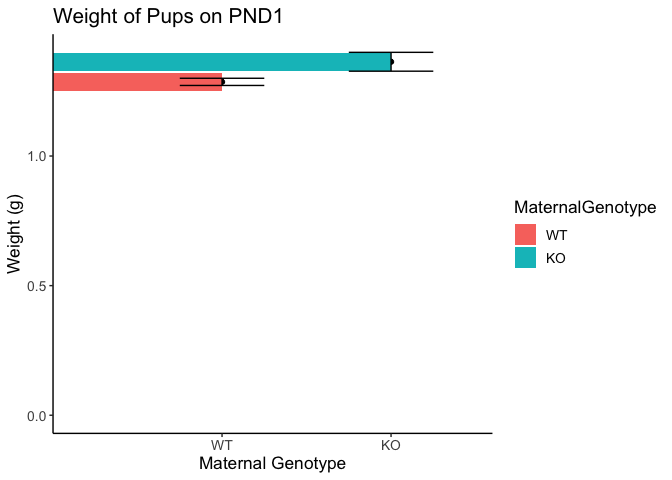
\includegraphics{figures/PUPweight_graphsPND1-2.png}

\begin{longtable}[]{@{}rrrrrrrrll@{}}
\caption{Welch's t-test for effects of maternal genotype on PND1
weights}\tabularnewline
\toprule
estimate & estimate1 & estimate2 & statistic & p.value & parameter &
conf.low & conf.high & method & alternative\tabularnewline
\midrule
\endfirsthead
\toprule
estimate & estimate1 & estimate2 & statistic & p.value & parameter &
conf.low & conf.high & method & alternative\tabularnewline
\midrule
\endhead
-0.078 & 1.29 & 1.36 & -1.99 & 0.09 & 6.43 & -0.171 & 0.016 & Welch Two
Sample t-test & two.sided\tabularnewline
\bottomrule
\end{longtable}

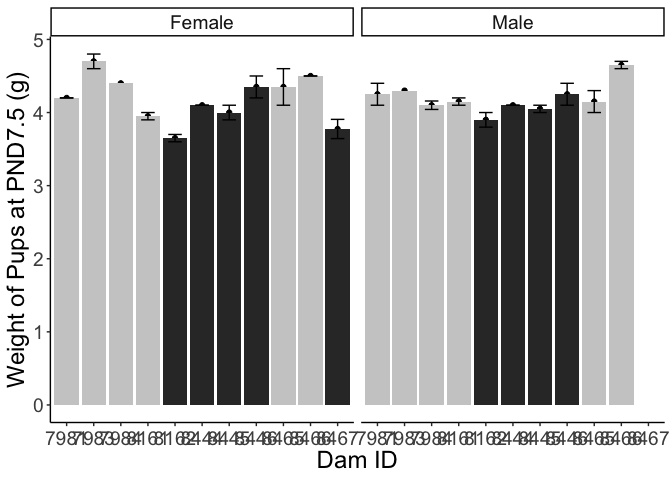
\includegraphics{figures/PUPweight_graphsPND7-1.png}
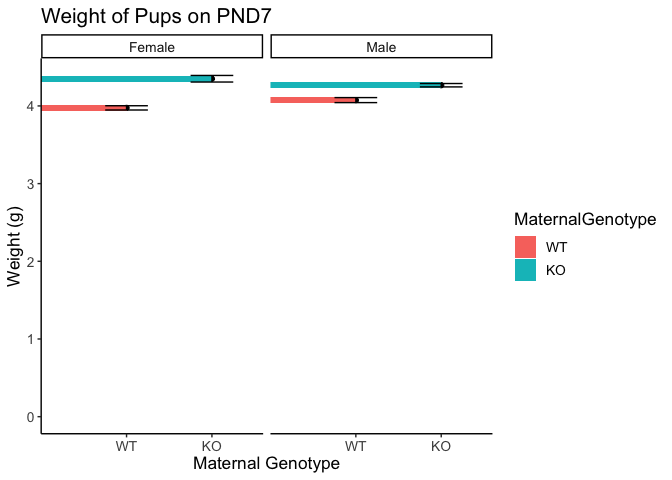
\includegraphics{figures/PUPweight_graphsPND7-2.png}

\begin{longtable}[]{@{}rrrrrrrrll@{}}
\caption{Welch's t-test for effects of maternal genotype on PND7 weights
in males}\tabularnewline
\toprule
estimate & estimate1 & estimate2 & statistic & p.value & parameter &
conf.low & conf.high & method & alternative\tabularnewline
\midrule
\endfirsthead
\toprule
estimate & estimate1 & estimate2 & statistic & p.value & parameter &
conf.low & conf.high & method & alternative\tabularnewline
\midrule
\endhead
-0.192 & 4.08 & 4.27 & -1.75 & 0.119 & 7.88 & -0.445 & 0.061 & Welch Two
Sample t-test & two.sided\tabularnewline
\bottomrule
\end{longtable}

\begin{longtable}[]{@{}rrrrrrrrll@{}}
\caption{Welch's t-test for effects of maternal genotype on PND7 weights
in females}\tabularnewline
\toprule
estimate & estimate1 & estimate2 & statistic & p.value & parameter &
conf.low & conf.high & method & alternative\tabularnewline
\midrule
\endfirsthead
\toprule
estimate & estimate1 & estimate2 & statistic & p.value & parameter &
conf.low & conf.high & method & alternative\tabularnewline
\midrule
\endhead
-0.375 & 3.98 & 4.35 & -2.32 & 0.047 & 8.39 & -0.745 & -0.005 & Welch
Two Sample t-test & two.sided\tabularnewline
\bottomrule
\end{longtable}

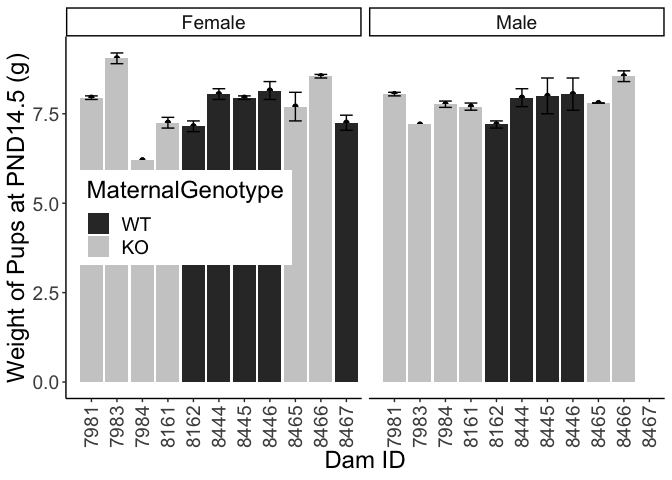
\includegraphics{figures/PUPweight_graphsPND14-1.png}
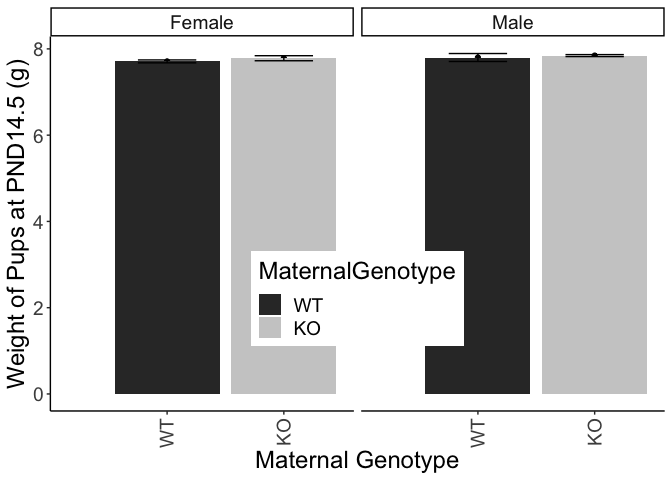
\includegraphics{figures/PUPweight_graphsPND14-2.png}

\begin{longtable}[]{@{}rrrrrrrrll@{}}
\caption{Welch's t-test for effects of maternal genotype on PND14
weights in males}\tabularnewline
\toprule
estimate & estimate1 & estimate2 & statistic & p.value & parameter &
conf.low & conf.high & method & alternative\tabularnewline
\midrule
\endfirsthead
\toprule
estimate & estimate1 & estimate2 & statistic & p.value & parameter &
conf.low & conf.high & method & alternative\tabularnewline
\midrule
\endhead
-0.044 & 7.8 & 7.84 & -0.164 & 0.874 & 7.06 & -0.683 & 0.594 & Welch Two
Sample t-test & two.sided\tabularnewline
\bottomrule
\end{longtable}

\begin{longtable}[]{@{}rrrrrrrrll@{}}
\caption{Welch's t-test for effects of maternal genotype on PND14
weights in females}\tabularnewline
\toprule
estimate & estimate1 & estimate2 & statistic & p.value & parameter &
conf.low & conf.high & method & alternative\tabularnewline
\midrule
\endfirsthead
\toprule
estimate & estimate1 & estimate2 & statistic & p.value & parameter &
conf.low & conf.high & method & alternative\tabularnewline
\midrule
\endhead
-0.073 & 7.71 & 7.78 & -0.159 & 0.878 & 7.37 & -1.15 & 1 & Welch Two
Sample t-test & two.sided\tabularnewline
{[}{]}(figures & /PUPweight\_g & raphsPND16-1 & .png)\textless{}!-- -- &
\textgreater{} {[}{]}(figu & res/PUPweigh & t\_graphsPND &
16-2.png)\textless{}!- & - --\textgreater{} &\tabularnewline
\bottomrule
\end{longtable}

\begin{longtable}[]{@{}rrrrrrrrll@{}}
\caption{Welch's t-test for effects of maternal genotype on PND16
weights in males}\tabularnewline
\toprule
estimate & estimate1 & estimate2 & statistic & p.value & parameter &
conf.low & conf.high & method & alternative\tabularnewline
\midrule
\endfirsthead
\toprule
estimate & estimate1 & estimate2 & statistic & p.value & parameter &
conf.low & conf.high & method & alternative\tabularnewline
\midrule
\endhead
0.033 & 8.43 & 8.39 & 0.107 & 0.918 & 6.28 & -0.719 & 0.785 & Welch Two
Sample t-test & two.sided\tabularnewline
\bottomrule
\end{longtable}

\begin{longtable}[]{@{}rrrrrrrrll@{}}
\caption{Welch's t-test for effects of maternal genotype on PND16
weights in females}\tabularnewline
\toprule
estimate & estimate1 & estimate2 & statistic & p.value & parameter &
conf.low & conf.high & method & alternative\tabularnewline
\midrule
\endfirsthead
\toprule
estimate & estimate1 & estimate2 & statistic & p.value & parameter &
conf.low & conf.high & method & alternative\tabularnewline
\midrule
\endhead
-0.127 & 8.19 & 8.32 & -0.282 & 0.785 & 8.03 & -1.16 & 0.908 & Welch Two
Sample t-test & two.sided\tabularnewline
\bottomrule
\end{longtable}

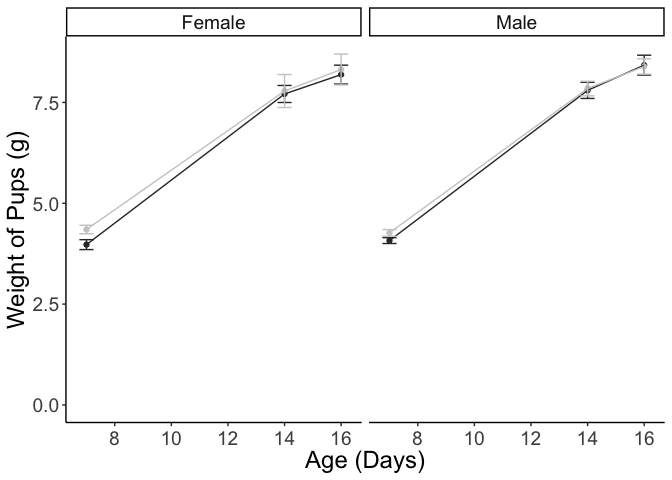
\includegraphics{figures/combined-weights_PND7_14_16-1.png}

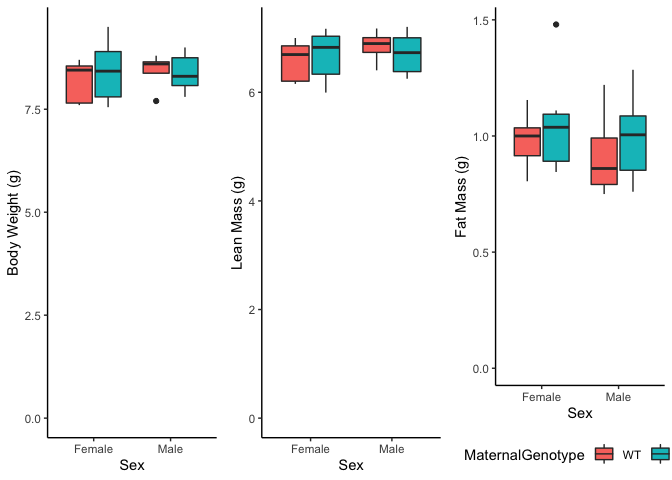
\includegraphics{figures/pupbodymass_PND16MRI-1.png}

\begin{longtable}[]{@{}rrrrrrrrll@{}}
\caption{Welch's t-test for effects of maternal genotype on aCasein milk
composition}\tabularnewline
\toprule
estimate & estimate1 & estimate2 & statistic & p.value & parameter &
conf.low & conf.high & method & alternative\tabularnewline
\midrule
\endfirsthead
\toprule
estimate & estimate1 & estimate2 & statistic & p.value & parameter &
conf.low & conf.high & method & alternative\tabularnewline
\midrule
\endhead
-0.011 & 8.43 & 8.44 & -0.045 & 0.965 & 12 & -0.556 & 0.534 & Welch Two
Sample t-test & two.sided\tabularnewline
\bottomrule
\end{longtable}

\begin{longtable}[]{@{}rrrrrrrrll@{}}
\caption{Welch's t-test for effects of maternal genotype on aCasein milk
composition}\tabularnewline
\toprule
estimate & estimate1 & estimate2 & statistic & p.value & parameter &
conf.low & conf.high & method & alternative\tabularnewline
\midrule
\endfirsthead
\toprule
estimate & estimate1 & estimate2 & statistic & p.value & parameter &
conf.low & conf.high & method & alternative\tabularnewline
\midrule
\endhead
-0.333 & 8.09 & 8.43 & -1.15 & 0.264 & 19.6 & -0.939 & 0.272 & Welch Two
Sample t-test & two.sided\tabularnewline
\bottomrule
\end{longtable}

\begin{longtable}[]{@{}rrrrrrrrll@{}}
\caption{Welch's t-test for effects of maternal genotype on aCasein milk
composition}\tabularnewline
\toprule
estimate & estimate1 & estimate2 & statistic & p.value & parameter &
conf.low & conf.high & method & alternative\tabularnewline
\midrule
\endfirsthead
\toprule
estimate & estimate1 & estimate2 & statistic & p.value & parameter &
conf.low & conf.high & method & alternative\tabularnewline
\midrule
\endhead
-0.094 & 0.922 & 1.02 & -0.683 & 0.511 & 9.68 & -0.401 & 0.214 & Welch
Two Sample t-test & two.sided\tabularnewline
\bottomrule
\end{longtable}

\begin{longtable}[]{@{}rrrrrrrrll@{}}
\caption{Welch's t-test for effects of maternal genotype on aCasein milk
composition}\tabularnewline
\toprule
estimate & estimate1 & estimate2 & statistic & p.value & parameter &
conf.low & conf.high & method & alternative\tabularnewline
\midrule
\endfirsthead
\toprule
estimate & estimate1 & estimate2 & statistic & p.value & parameter &
conf.low & conf.high & method & alternative\tabularnewline
\midrule
\endhead
-0.074 & 0.985 & 1.06 & -0.863 & 0.4 & 16.9 & -0.256 & 0.107 & Welch Two
Sample t-test & two.sided\tabularnewline
\bottomrule
\end{longtable}

\begin{longtable}[]{@{}rrrrrrrrll@{}}
\caption{Welch's t-test for effects of maternal genotype on aCasein milk
composition}\tabularnewline
\toprule
estimate & estimate1 & estimate2 & statistic & p.value & parameter &
conf.low & conf.high & method & alternative\tabularnewline
\midrule
\endfirsthead
\toprule
estimate & estimate1 & estimate2 & statistic & p.value & parameter &
conf.low & conf.high & method & alternative\tabularnewline
\midrule
\endhead
0.089 & 6.84 & 6.75 & 0.506 & 0.62 & 15.3 & -0.286 & 0.464 & Welch Two
Sample t-test & two.sided\tabularnewline
\bottomrule
\end{longtable}

\begin{longtable}[]{@{}rrrrrrrrll@{}}
\caption{Welch's t-test for effects of maternal genotype on aCasein milk
composition}\tabularnewline
\toprule
estimate & estimate1 & estimate2 & statistic & p.value & parameter &
conf.low & conf.high & method & alternative\tabularnewline
\midrule
\endfirsthead
\toprule
estimate & estimate1 & estimate2 & statistic & p.value & parameter &
conf.low & conf.high & method & alternative\tabularnewline
\midrule
\endhead
-0.171 & 6.51 & 6.68 & -0.875 & 0.391 & 21.7 & -0.576 & 0.234 & Welch
Two Sample t-test & two.sided\tabularnewline
\bottomrule
\end{longtable}

\end{document}
